\documentclass{article}

\usepackage[nonatbib, final]{neurips}
\usepackage[numbers]{natbib}

\makeatletter
\renewcommand{\@noticestring}{
  \centering
  
}
\makeatother

\usepackage[export]{adjustbox}
\usepackage[ruled]{algorithm2e}
\usepackage[inline, shortlabels]{enumitem}
\usepackage[T1]{fontenc}
\usepackage{hyperref}
\usepackage{microtype}
\usepackage{pifont}
\usepackage{xcolor}
\usepackage{xurl}
% Figures and Tables
\usepackage{graphicx}
\usepackage{booktabs}
\usepackage{tabularray}
% Monospaced Code Blocks
\usepackage{listings}
% Math Packages
\usepackage{amsmath, amsfonts}
\usepackage{nicefrac}

\UseTblrLibrary{booktabs}

\lstset{
  backgroundcolor=\color{white},   % choose the background color; you must add \usepackage{color} or \usepackage{xcolor}; should come as last argument
  basicstyle=\ttfamily,            % the size of the fonts that are used for the code
  breakatwhitespace=false,         % sets if automatic breaks should only happen at whitespace
  breaklines=true,                 % sets automatic line breaking
  captionpos=b,                    % sets the caption-position to bottom
  columns=fullflexible,            % reduce the column spacing
  commentstyle=\color{gray},       % comment style
  deletekeywords={},               % if you want to delete keywords from the given language
  escapeinside={\%*}{*)},          % if you want to add LaTeX within your code
  extendedchars=true,              % lets you use non-ASCII characters; for 8-bits encodings only, does not work with UTF-8
  frame=none,                      % adds no frame around the code
  keepspaces=true,                 % keeps spaces in text, useful for keeping indentation of code (possibly needs columns=flexible)
  keywordstyle=\color{blue},       % keyword style
  language=C++,                    % the language of the code
  morekeywords={},                 % if you want to add more keywords to the set
  numbers=none,                    % where to put the line-numbers; possible values are (none, left, right)
  numbersep=5pt,                   % how far the line-numbers are from the code
  numberstyle=\color{black},       % the style that is used for the line-numbers
  rulecolor=\color{black},         % if not set, the frame-color may be changed on line-breaks within not-black text (e.g. comments (green here))
  showspaces=false,                % show spaces everywhere adding particular underscores; it overrides 'showstringspaces'
  showstringspaces=false,          % underline spaces within strings only
  showtabs=false,                  % show tabs within strings adding particular underscores
  stepnumber=1,                    % the step between two line-numbers. If it's 1, each line will be numbered
  stringstyle=\color{red},         % string literal style
  tabsize=4,                       % sets default tabsize to 4 spaces
}

\makeatletter
\newcommand{\ssymbol}[1]{\@fnsymbol{#1}}
\newcommand{\romanNumeral}[1]{\expandafter\@slowromancap\romannumeral #1@}
\makeatother

\setlength{\textfloatsep}{12pt plus 2pt minus 2pt}

\usepackage{physics}
\usepackage{mathtools}
\DeclarePairedDelimiter\p{(}{)}
\DeclarePairedDelimiter\n{|}{|}
\DeclarePairedDelimiter\B{[}{]}

\title{Fine-Tuning, Vision-Language Models, and Test-Time Compute}

\author{
    Ali Hasnain \\
    28100341 \\
}

\begin{document}

\maketitle
\suppressfloats[t]

\begin{abstract}
We study three ways of adapting and extending small language models on Tesla T4 GPUs. \emph{Fine-tuning:} adapting Qwen3-0.6B to MetaMathQA, full fine-tuning raises GSM8K accuracy from 43.4\% to 64.4\% but degrades HellaSwag and BoolQ. L2-SP matches this gain (65.0\%) with roughly 40\% less parameter displacement, and LoRA ($r{=}16$) reaches 62.2\% while training only 1.67\% of the parameters and improving every retention benchmark. OPLoRA nearly eliminates interference with the protected subspace but does not outperform LoRA and is the slowest adapter method. \emph{Vision-language models:} connecting a frozen SigLIP encoder to a frozen Qwen3-0.6B through an MLP connector and LoRA, the model reaches 69.5\% on annotation-derived grounding and 56.8\% on VQAv2. Accuracy falls to 11.7\% and 25.4\% when the image is swapped for its complement, so the model is using the image. Image sensitivity emerges mainly during visual instruction tuning rather than caption alignment. Pooling to 49 visual tokens halves training time at comparable accuracy but increases reliance on language priors. \emph{Test-time compute:} with 32 rollouts per question, self-consistency improves MATH from 63.6\% to 74.0\% and MathVista from 53.9\% to 63.2\%, and rank-weighted consensus on self-certainty adds a further 1.6 pp on MATH. Because oracle coverage reaches about 90\%, selection rather than generation is the main bottleneck. The best adaptive stopping policy on each dataset comes within 0.3 pp of fixed 32-sample accuracy with roughly half the tokens, whereas, under a matched live budget, neither parallel sampling nor sequential refinement beats a single generation. Code and results: \url{https://github.com/alihasnaink/finetune-ground-scale}.
\end{abstract}

\section{Fine-Tuning}
\label{sec:finetuning}

\subsection{Introduction}
\label{sec:finetuning-intro}

Fine-tuning adapts pretrained models to specialized tasks but can compromise previously acquired capabilities. We compare Full FT, which updates all parameters; L2-SP, which penalizes deviations from pretrained weights; LoRA, which learns low-rank adapters; and OPLoRA, which constrains adapter updates to reduce interference with dominant pretrained subspaces.

We fine-tune Qwen3-0.6B on MetaMathQA and evaluate mathematical performance on GSM8K and retention on HellaSwag, BoolQ, and ARC-Easy. We investigate the effects of regularization, adapter rank, and orthogonal protection on performance, retention, and computational cost.

\subsection{Experimental Setup}
\label{sec:finetuning-setup}

We use Qwen3-0.6B (596M parameters) and the first 40,000 eligible MetaMathQA examples, training for 1,250 updates (effective batch size 32). Five configurations are evaluated: Full FT, Full FT with L2-SP ($\lambda=10^{-3}$), LoRA (ranks 4 and 16), and OPLoRA (rank 16, protecting the top 128 singular directions). Training was performed on a Tesla T4 using FP16 mixed precision, dynamic loss scaling, and FP32 master weights. Evaluation uses GSM8K (1,319 questions) for mathematical performance and HellaSwag, BoolQ, and ARC-Easy for capability retention. Full FT was evaluated at updates 625 and 1,250, while the remaining methods were evaluated only at the final update. We additionally measured parameter displacement, subspace interference, and activation changes using \texttt{down\_proj} in layers 0, 13, and 27, alongside qualitative comparisons of model responses.

\subsection{Results}
\label{sec:finetuning-results}

\paragraph{Benchmark results.}
Full fine-tuning demonstrated the strongest progression on GSM8K, improving from 43.37\% at baseline to 57.32\% at the midpoint and 64.44\% in the final checkpoint (+21.08 percentage points; Table~\ref{tab:t1-benchmarks}). However, this improvement came with regressions on HellaSwag ($-1.26$ pp) and BoolQ ($-3.09$ pp). L2-SP and LoRA offered better retention of general capabilities, with LoRA $r{=}16$ achieving the highest BoolQ score (72.60\%, +8.23 pp). Overall, OPLoRA achieved improvements across all four benchmarks, although it did not outperform standard LoRA $r{=}16$.

\paragraph{Learning and regularization.}
The training-loss plot (Figure~\ref{fig:t1-loss}) shows rapid convergence during the initial updates, followed by a relatively stable plateau across all five runs. Full FT and L2-SP achieved the lowest final SFT loss (0.188), while LoRA $r{=}4$ had the highest (0.216; Table~\ref{tab:t1-displacement}). L2-SP reduced parameter displacement $\|\theta-\theta_0\|_2$ from 10.67 to 6.28, reducing the penalty $\Omega=\tfrac12\|\theta-\theta_0\|_2^2$ from 56.9 to 19.7. In contrast, LoRA $r{=}16$ exhibited the largest displacement (13.32), suggesting that a higher adapter rank does not necessarily constrain the magnitude of parameter updates.

\paragraph{Training resources.}
Full FT and L2-SP updated 596M parameters, whereas LoRA and OPLoRA trained only 2.5M--10.1M parameters (0.42--1.67\% of the full model; Table~\ref{tab:t1-resources}). LoRA $r{=}4$ required the least GPU memory (4.7 GB), compared with 11.2 GB for Full FT. However, training times were relatively close: 2.35 hours for Full FT versus 2.60 hours for LoRA $r{=}4$. OPLoRA was the most expensive adapter-based approach, taking 3.27 hours; the one-off basis computation took only 32 s, so most of the overhead comes from projecting the adapter factors at every update.

\paragraph{Model diagnostics.}
The diagnostics in Table~\ref{tab:t1-diagnostics} reveal differences in how each approach modifies the pretrained model. L2-SP produced smaller relative parameter updates than Full FT, consistent with its regularization objective. OPLoRA achieved near-zero subspace interference, indicating that its updates were effectively excluded from the measured dominant output singular subspaces. Activation correction ratios were higher for mathematical probes in layers 0 and 13, particularly for LoRA $r{=}4$, suggesting stronger changes in mathematical activations relative to non-mathematical ones; in layer 27 the ratio is below one for every method. However, these measurements describe selected layers and probes; they cannot independently establish that a particular modification caused the observed benchmark improvements.

\paragraph{Qualitative findings.}
Manual annotation of 42 responses (Table~\ref{tab:t1-annotation}) revealed differences that benchmark scores alone could not capture. Full FT exhibited repetitive mathematical-style continuations, including responses that reached the 512-token generation limit. L2-SP reduced some of these behaviors but retained occasional mathematical framing in ordinary responses. LoRA $r{=}4$ generally maintained coherent and concise responses, while higher-rank LoRA occasionally exhibited repetition and formatting failures. OPLoRA maintained relatively strong coherence and formatting performance. The selected examples in Table~\ref{tab:t1-examples} illustrate these behaviors using identical prompts and output formats, although the small, fixed annotation subset is insufficient to establish their prevalence across general usage.

\begin{table}[t]
\centering
\small
\caption{Task 1 benchmark scores (\%), with the change from baseline in pp. GSM8K: flexible-extract exact match; HellaSwag, ARC-Easy: normalized accuracy; BoolQ: accuracy.}
\label{tab:t1-benchmarks}
\begin{adjustbox}{max width=\linewidth}
\begin{tabular}{lcccc}
\toprule
Condition & GSM8K & HellaSwag & BoolQ & ARC-Easy \\
\midrule
Baseline & 43.37 & 47.32 & 64.37 & 56.06 \\
\midrule
Full FT (mid) & 57.32 \,(+13.95) & 45.69 \,(-1.63) & 60.80 \,(-3.58) & 62.04 \,(+5.98) \\
Full FT (final) & 64.44 \,(+21.08) & 46.06 \,(-1.26) & 61.28 \,(-3.09) & 63.47 \,(+7.41) \\
\midrule
L2-SP & 64.97 \,(+21.61) & 46.50 \,(-0.82) & 67.06 \,(+2.69) & 63.22 \,(+7.15) \\
LoRA $r{=}4$ & 60.12 \,(+16.76) & 47.40 \,(+0.08) & 66.39 \,(+2.02) & 63.22 \,(+7.15) \\
LoRA $r{=}16$ & 62.24 \,(+18.88) & 47.56 \,(+0.24) & 72.60 \,(+8.23) & 64.06 \,(+8.00) \\
OPLoRA & 62.17 \,(+18.80) & 47.39 \,(+0.07) & 72.08 \,(+7.71) & 63.13 \,(+7.07) \\
\bottomrule
\end{tabular}
\end{adjustbox}
\end{table}


\subsection{Discussion and Interpretation}
\label{sec:finetuning-discussion}

\paragraph{Forgetting and retention.}
Catastrophic forgetting \citep{kirkpatrick2017overcoming} occurs when adapting to a new task interferes with parameters supporting existing capabilities. This explains the Full FT results: mathematical performance improved substantially (+21.08 pp on GSM8K), but HellaSwag and BoolQ declined. In contrast, L2-SP and LoRA largely preserved or improved performance on the retention benchmarks (L2-SP's only regression is $-0.82$ pp on HellaSwag), suggesting that specialization does not necessarily require sacrificing general capabilities.

\paragraph{Starting-point regularization.}
L2-SP regularization \citep{li2018l2sp} penalizes deviations from pretrained parameters, encouraging the model to preserve existing representations. This is consistent with L2-SP achieving smaller parameter displacement while maintaining strong mathematical performance.

\paragraph{Adapter rank.}
Low-Rank Adaptation \citep{hu2022lora} restricts parameter updates to low-rank matrices. Increasing rank provides greater adaptation capacity, consistent with the improved GSM8K and BoolQ results of LoRA $r{=}16$ compared with $r{=}4$.

\paragraph{Orthogonal protection.}
Orthogonal protection \citep{farajtabar2020ogd} restricts updates to directions orthogonal to a protected subspace, potentially reducing interference with existing knowledge. However, parameter-space orthogonality does not guarantee better downstream performance, as demonstrated by OPLoRA.

\paragraph{Displacement versus behavior.}
Parameter displacement alone does not determine behavioral changes. This explains why different parameter updates can produce different effects on mathematical and non-mathematical inputs. The activation correction measurements provide evidence of this input-dependent behavior, while subspace interference describes the geometry of parameter updates. Neither measurement independently establishes the cause of benchmark improvements.

\paragraph{Efficiency.}
LoRA's efficiency follows from its low-rank parameterization, which reduces trainable parameters from $d_\text{out}d_\text{in}$ to $r(d_\text{out}+d_\text{in})$. This substantially reduces optimizer and gradient memory requirements. The experiments support this theoretical advantage: LoRA $r{=}16$ trained only 1.67\% of the model parameters while achieving strong mathematical performance and general capability retention. In comparison, L2-SP still updates all model parameters despite restricting their displacement. OPLoRA introduces additional computational overhead through basis construction and the per-update projection of its adapter factors. These findings demonstrate that parameter efficiency does not necessarily translate into reductions in training time: LoRA $r{=}4$ was in fact slightly slower than Full FT (2.60 vs.\ 2.35 hours), since forward propagation and activation computation through the full model remain necessary.

\paragraph{Qualitative behavior.}
Full FT produced repetitive mathematical-style continuations, while L2-SP exhibited occasional mathematical framing. LoRA and OPLoRA generally maintained stronger coherence, although formatting failures and repetition were still observed. These findings highlight the distinction between retaining a capability and appropriately activating it. Qualitative evaluation therefore complements benchmark testing by identifying behavioral changes that accuracy metrics cannot capture. However, the 42-response subset provides illustrative rather than statistically representative evidence.

\section{Vision-Language Models}
\label{sec:vlm}

\subsection{Introduction}
\label{sec:vlm-intro}

Vision-Language Models (VLMs) combine visual and linguistic information to answer questions about images, requiring the model to ground its responses in visual evidence rather than relying solely on language priors. We connect a pretrained SigLIP vision encoder to Qwen3-0.6B through a trainable connector, training it through caption alignment and visual question answering.

The experiments examine caption-based alignment, annotation-derived visual grounding, and VQA fine-tuning using complementary image pairs. We also use image controls to assess whether the model genuinely relies on visual evidence when answering questions.

\subsection{Experimental Setup}
\label{sec:vlm-setup}

We combine a frozen SigLIP-Base-Patch16-224 vision encoder with a frozen Qwen3-0.6B language model through a trainable two-layer MLP connector ($768 \rightarrow 1024 \rightarrow 1024$). We compare configurations using 196 visual tokens ($14\times14$ patches) and 49 tokens ($2\times2$ patch pooling). Training follows three stages: caption alignment (2,250 updates), visual instruction tuning (1,500 updates), and natural VQA (750 updates). The data comprises 18,000 COCO caption examples, annotation-derived presence and counting pairs, and 1,536 VQAv2 complementary training pairs. Evaluation uses 96 VQAv2 test pairs and 64 annotation-derived test pairs, comparing correct-image, complementary-image, mismatched-image, and no-image conditions. The connector contained approximately 1.84M parameters, while LoRA adapters were introduced only in the second and third training stages. Training used an effective batch size of 16, with FP16 autocasting and FP32 trainable parameters. We evaluated both visual-token configurations using greedy decoding with a 16-token output limit. Results were compared using 4,000 pair-level bootstrap resamples to obtain 95\% confidence intervals.

\subsection{Results}
\label{sec:vlm-results}

\paragraph{Training dynamics.}
Figure~\ref{fig:t2-curves} shows that caption alignment (stage 1) reduces the development caption loss from 5.52 to 2.29, which then stays flat (2.31--2.33) through the later stages, so caption replay prevents forgetting. However, stage 1 alone produces almost no image sensitivity: the image-swap penalty $\Delta$NLL on grounding stays between 0.3 and 0.6 for the 196-token model (below 1.0 for the 49-token model). Sensitivity emerges in stage 2, when visual instruction tuning and LoRA are introduced: grounding $\Delta$NLL rises from 0.57 to 2.70 at the first stage-2 evaluation and to 3.85 by the end of the stage, while correct-image answer NLL falls from 5.85 to about 0.6. The 49-token model diverges here: its no-image grounding NLL collapses from 11.0 to 1.3, whereas the 196-token model's remains at 6.7, consistent with the 49-token model's higher no-image accuracy. The shift to natural VQA in stage 3 briefly reduces $\Delta$NLL (3.85 to 2.14) before it partly recovers (3.14).

\paragraph{Image grounding and overall accuracy.}
With 196 visual tokens, the model achieves 69.5\% accuracy on Grounding and 56.8\% on VQAv2 when given the correct image (Table~\ref{tab:t2-main}). Replacing the image with a complementary image reduces accuracy to 11.7\% and 25.4\%, respectively. Mismatched images also reduce performance, confirming that predictions are influenced by visual content rather than relying entirely on language priors. The 49-token model achieves comparable correct-image accuracy (72.7\% Grounding and 52.6\% VQAv2), suggesting that reducing visual tokens does not necessarily compromise grounding performance.

\paragraph{Performance without images.}
The 196-token model achieves 0\% strict accuracy without an image because it then answers in full sentences (e.g.\ ``No, the image does not contain a knife.''); scoring the leading yes/no or number instead gives 24.2\% on Grounding and 18.8\% on VQAv2 (lenient accuracy, Table~\ref{tab:t2-main}). The 49-token model, which keeps answering tersely, retains 33.6\% Grounding and 31.4\% VQAv2 accuracy without images, close to chance on presence (50.0\%) and yes/no questions (56.2\%; Table~\ref{tab:t2-bytype}). This suggests that the smaller visual representation may encourage greater reliance on learned language priors, potentially at the expense of visual grounding.

\paragraph{Question-type performance.}
Grounding performance is strongest on presence questions (approximately 89--91\%) but weaker on counting questions (50--55\%; Table~\ref{tab:t2-bytype}). On VQAv2, yes/no questions achieve better accuracy (approximately 68--70\%) than numerical and other questions. Complementary-image accuracy remains substantially lower across question types, indicating that the model struggles when the relevant visual evidence is replaced.

\paragraph{Correct-image advantage and pair diagnostics.}
The correct image provides a substantial advantage over complementary images: 57.8 and 60.9 percentage points for the 196- and 49-token Grounding models, respectively (Table~\ref{tab:t2-advantages}). On VQAv2, the corresponding advantages are 31.4 and 27.8 points. Pair accuracy shows similar trends. Furthermore, under complementary swaps, the model follows the partner image's answer in 69.5--72.7\% of Grounding cases, demonstrating sensitivity to changes in visual evidence. The positive NLL advantages and their bootstrap confidence intervals, all of which exclude zero, further support the reliability of these differences.

\paragraph{Qualitative findings.}
The selected examples in Table~\ref{tab:t2-examples} illustrate three behaviors: successful grounding when both images support correct answers, image-insensitive predictions where swapping images does not change the response, and image-sensitive errors where the model's answer changes with the image but is still wrong. For example, the model correctly counts the trains in both images of a pair; for the kites pair its answer changes with the image, but it answers 4 where the reference is 3. Conversely, it consistently predicts the shirt color as white despite one reference indicating pink. These examples highlight both effective visual conditioning and remaining grounding failures.

\paragraph{Computational efficiency.}
Each run used a single Tesla T4 GPU (Table~\ref{tab:t2-resources}). Reducing visual tokens from 196 to 49 approximately halves training time: total stage training decreases from 93.59 to 44.52 minutes. Peak training memory also decreases slightly, from 1.60 GB to 1.51 GB. The model uses 1.84M trainable parameters during caption alignment and 6.42M during subsequent stages, including LoRA adapters. Shared SigLIP feature caching takes only 2.73 minutes for 9,255 images, making the overall training pipeline relatively lightweight.

\begin{table}[t]
\centering
\small
\caption{Task 2 held-out accuracy (\%) under four image conditions (64 grounding, 96 VQAv2 pairs). Lenient: leading yes/no or number of a sentence answer; pair: both images of a pair correct. CIs and NLL in Table~\ref{tab:t2-final}.}
\label{tab:t2-main}
\begin{adjustbox}{max width=\linewidth}
\begin{tabular}{llcccccc}
\toprule
Tokens & Suite & Correct & Complementary & Mismatched & No image & No image (lenient) & Pair \\
\midrule
196 & Grounding & 69.5 & 11.7 & 37.5 & 0.0 & 24.2 & 53.1 \\
196 & VQAv2 & 56.8 & 25.4 & 34.3 & 0.0 & 18.8 & 26.0 \\
\midrule
49 & Grounding & 72.7 & 11.7 & 32.8 & 33.6 & 33.6 & 56.2 \\
49 & VQAv2 & 52.6 & 24.7 & 31.5 & 31.4 & 31.4 & 25.0 \\
\bottomrule
\end{tabular}
\end{adjustbox}
\end{table}


\subsection{Discussion and Interpretation}
\label{sec:vlm-discussion}

\paragraph{Learning a visual interface.}
The three-stage training (caption alignment, visual instruction tuning, and natural VQA) progressively establishes visual-language alignment and transfers it into question-answering capabilities. However, capabilities do not transfer uniformly: counting and numerical reasoning remain weaker than basic visual recognition.

\paragraph{Grounding and generalization.}
The model demonstrates meaningful dependence on visual evidence. With 196 tokens, correct-image accuracy reaches 69.5\% on Grounding and 56.8\% on VQAv2, dropping substantially under complementary and mismatched images. Grounding performance is stronger on annotation-derived questions than natural VQA (although the two suites use different metrics), suggesting difficulties generalizing to less structured language. The 49-token model's higher no-image accuracy also suggests greater reliance on linguistic priors.

\paragraph{Measuring image use.}
Reference NLL, generated-answer accuracy, pair-level diagnostics, and qualitative examples provide consistent evidence of visual conditioning. Complementary-image swaps frequently cause predictions to follow the partner image's answer, supporting image sensitivity. However, image sensitivity does not necessarily imply correct visual understanding. This is particularly important when interpreting counterfactual evaluations.

\paragraph{Capabilities and cost.}
The model learns caption alignment and visual question answering using a relatively lightweight connector and LoRA-based architecture. Reducing visual tokens from 196 to 49 cuts training time from 93.59 to 44.52 minutes and evaluation time from 1.61 to 0.75 minutes on a Tesla T4. Feature caching takes just 2.73 minutes for 9,255 images. These savings come with a potential trade-off in visual grounding, as the 49-token model relies more heavily on language priors.

\section{Test-Time Compute}
\label{sec:tts}

\subsection{Introduction}
\label{sec:tts-intro}

Test-Time Compute (TTC) explores how additional computation during inference can improve model performance without retraining. We investigate parallel sampling, best-of-N selection, self-consistency, and sequential refinement. Using supplied LLM and VLM rollouts, we compare selection strategies, confidence and visual-grounding signals, parallel generation against sequential refinement, and adaptive sampling to study the trade-off between accuracy and computational cost.

\subsection{Experimental Setup}
\label{sec:tts-setup}

We use 32 sampled rollouts per question from Qwen2.5-3B-Instruct on a 1,000-question MATH subset and Qwen2.5-VL-3B-Instruct on 1,000 MathVista questions. The supplied generations use temperature 0.7 and a 2,048-token limit. We reserve 200 questions per dataset for development and 800 for held-out evaluation. Offline experiments compare candidate budgets of 1, 2, 4, 8, 16, and 32 across ten rollout orders, using selection methods such as self-consistency, self-certainty, log-probability, and VisConf with rank-weighted consensus. A live experiment on 50 MATH questions compares one 3,072-token response, three parallel 1,024-token responses, and sequential refinement with a 1,024-token initial response followed by up to 2,048 tokens. Finally, adaptive stopping is evaluated at 4, 8, and 16 rollouts, with 32 as the maximum budget. All experiments compare accuracy against computational cost.

\subsection{Results}
\label{sec:tts-results}

\paragraph{Sampling and selection.}
Increasing the number of sampled answers improves accuracy on both MATH and MathVista when the answer is chosen by consensus (Figure~\ref{fig:t3-n}, Table~\ref{tab:t3-methods}); selecting the single highest-scoring rollout gains little or even declines as $N$ grows. Self-consistency raises accuracy from 63.6\% to 74.0\% on MATH and 53.9\% to 63.2\% on MathVista at $N{=}32$. Quality-aware selection (RWC) further improves these to 75.6\% and 64.5\%; the gain over self-consistency is significant on MATH (+1.6 pp, 95\% CI [0.5, 2.7]) but not on MathVista (+1.3 pp, [$-0.1$, 2.8]; Table~\ref{tab:t3-boot}). Oracle coverage reveals that many remaining errors arise from selecting incorrect candidates rather than failing to generate a correct one: at $N{=}32$ only 8.6\% (MATH) and 10.5\% (MathVista) of questions have no correct candidate, whereas self-consistency misses an available correct answer on 17.4\% and 26.3\% (Table~\ref{tab:t3-decomp}).

\paragraph{Signal analysis.}
Self-certainty and visual-confidence signals provide useful information about candidate quality, while response length is only weakly correlated with correctness (Spearman $-0.08$ on MATH and $-0.05$ on MathVista; Table~\ref{tab:t3-signals}). Combining confidence with consensus improves selection over choosing the highest-scoring rollout, particularly on MathVista (VisConf: 57.8\% $\rightarrow$ 64.5\%; self-certainty: 54.6\% $\rightarrow$ 63.8\% at $N{=}32$). However, token-level fusion offers no meaningful advantage over trajectory-level fusion: it is slightly worse (e.g.\ $-1.5$ pp for highest-score selection at $N{=}32$, Table~\ref{tab:t3-boot}), consistent with confidence and visual engagement being negatively correlated within rollouts (mean $-0.20$; Figure~\ref{fig:t3-traj}).

\paragraph{Live inference.}
Single generation achieves the highest accuracy (66\%) on the 50-question evaluation, compared with 62\% for parallel sampling and refinement (Table~\ref{tab:t3-live}). Parallel sampling is the most expensive, taking 86.3 seconds per question, while refinement takes 53.5 seconds and single generation 34.7 seconds. Neither provides a statistically significant improvement over single generation, suggesting that additional inference computation does not automatically improve accuracy.

\paragraph{Adaptive inference.}
Adaptive stopping achieves accuracy close to fixed 32-sample self-consistency while substantially reducing computational costs (Figure~\ref{fig:t3-cost}, Table~\ref{tab:t3-adaptive}). On MATH, agreement-based stopping achieves 73.7\% accuracy using approximately 10,112 tokens instead of 21,347. On MathVista, quality-aware stopping achieves 63.1\% using 3,967 tokens instead of 8,898. However, premature stopping can prevent potentially correct answers from emerging through further sampling.

\paragraph{Qualitative findings.}
Examples demonstrate that confidence-aware selection can recover correct minority answers, but can also favor confidently incorrect responses (Table~\ref{tab:t3-cases}). Similarly, adaptive stopping occasionally terminates too early, while a single round of refinement never corrected an initial mistake.

\begin{table}[t]
\centering
\small
\caption{Held-out accuracy (\%; 800 questions, 10 orders) by budget $N$; at $N{=}1$ all methods equal FirstAns (63.6, 53.9). Bold: best per column; last row: oracle coverage. Curves in Figure~\ref{fig:t3-n}.}
\label{tab:t3-methods}
\begin{adjustbox}{max width=\linewidth}
\begin{tabular}{lcccccccccc}
\toprule
 & \multicolumn{5}{c}{MATH (Qwen2.5-3B)} & \multicolumn{5}{c}{MathVista (Qwen2.5-VL-3B)} \\
\cmidrule(lr){2-6}\cmidrule(lr){7-11}
Method & $N{=}2$ & $N{=}4$ & $N{=}8$ & $N{=}16$ & $N{=}32$ & $N{=}2$ & $N{=}4$ & $N{=}8$ & $N{=}16$ & $N{=}32$ \\
\midrule
FirstAns & 63.6 & 63.6 & 63.6 & 63.6 & 63.6 & 53.9 & 53.9 & 53.9 & 53.9 & 53.9 \\
Self-consistency & 63.6 & 69.0 & 71.6 & 73.2 & 74.0 & 53.9 & \textbf{58.7} & 60.8 & 62.5 & 63.2 \\
Max mean log-prob & 65.9 & 66.8 & 67.4 & 66.4 & 64.0 & 54.8 & 54.3 & 52.7 & 50.8 & 48.1 \\
Max self-certainty & \textbf{66.5} & 68.6 & 70.2 & 70.6 & 70.6 & 55.2 & 55.1 & 55.2 & 55.1 & 54.6 \\
Self-certainty + RWC & \textbf{66.5} & \textbf{69.7} & \textbf{72.8} & \textbf{74.5} & \textbf{75.6} & 55.2 & 57.0 & 60.7 & 62.2 & 63.8 \\
Shortest (length control) & 64.8 & 64.9 & 64.1 & 63.1 & 62.4 & 55.4 & 55.0 & 54.5 & 54.4 & 53.7 \\
\midrule
Max vision $V$ & -- & -- & -- & -- & -- & 55.3 & 54.5 & 53.9 & 53.6 & 53.6 \\
Vision + RWC & -- & -- & -- & -- & -- & 55.3 & 57.5 & 60.5 & 62.3 & 63.9 \\
Max VisConf $Z$ & -- & -- & -- & -- & -- & \textbf{56.2} & 56.7 & 56.9 & 57.2 & 57.8 \\
VisConf + RWC & -- & -- & -- & -- & -- & \textbf{56.2} & 58.5 & \textbf{61.5} & \textbf{63.3} & \textbf{64.5} \\
Max token fusion $Z^\text{tok}$ & -- & -- & -- & -- & -- & 56.0 & 56.6 & 56.0 & 55.9 & 56.2 \\
Token fusion + RWC & -- & -- & -- & -- & -- & 56.0 & 58.5 & 61.2 & 63.0 & 63.9 \\
\midrule
\emph{Oracle coverage} & \emph{72.3} & \emph{79.0} & \emph{84.4} & \emph{88.3} & \emph{91.4} & \emph{66.8} & \emph{76.2} & \emph{82.9} & \emph{87.0} & \emph{89.5} \\
\bottomrule
\end{tabular}
\end{adjustbox}
\end{table}


\begin{table}[t]
\centering
\small
\caption{Live comparison on 50 MATH questions (same 3{,}072-token allowance; per-question means, shared initial response charged to both parallel and refinement). Initial accuracy 62\%, parallel oracle 68\%. Revisions: W$\to$C 0, C$\to$W 0, C$\to$C 31, W$\to$W 19. Bootstrap: parallel $-$ single -4 pp [-16, 8], refinement $-$ single -4 pp [-14, 8].}
\label{tab:t3-live}
\begin{adjustbox}{max width=\linewidth}
\begin{tabular}{lcccccccc}
\toprule
Strategy & Acc.\ (\%) & No answer (\%) & Extracted (\%) & Truncated (\%) & In tokens & Out tokens & Time (s) & Peak mem (GB) \\
\midrule
Single (1$\times$3{,}072) & 66.0 & 4.0 & 96.0 & 4.0 & 108 & 738 & 34.7 & 6.09 \\
Parallel (3$\times$1{,}024) + SC & 62.0 & 10.0 & 86.7 & 14.0 & 325 & 1878 & 86.3 & 5.94 \\
Refinement (1{,}024 + 2{,}048) & 62.0 & 0.0 & 95.0 & 5.0 & 870 & 1142 & 53.5 & 6.17 \\
\bottomrule
\end{tabular}
\end{adjustbox}
\end{table}


\begin{table}[t]
\centering
\small
\caption{Adaptive sampling (held-out; thresholds frozen on dev as the cheapest setting within 1 pp of fixed-32 self-consistency). Stops: \% of runs stopping at $n{=}$4 / 8 / 16 / 32. Last column: difference to fixed-32 self-consistency (pp, 95\% CI).}
\label{tab:t3-adaptive}
\begin{adjustbox}{max width=\linewidth}
\begin{tabular}{llcccccc}
\toprule
 & Policy & Setting & Acc.\ (\%) & Tokens & Rollouts & Stops (\%) & $\Delta$ vs SC@32 \\
\midrule
MATH & Fixed SC, $N{=}16$ & -- & 73.2 & 10{,}669 & 16 & -- & -- \\
 & Fixed SC, $N{=}32$ & -- & 74.0 & 21{,}347 & 32 & -- & -- \\
 & Agreement stop & $\tau{=}0.625$ & 73.7 & 10{,}112 & 11.8 & 67 / 5 / 1 / 26 & -0.29 [-0.68, 0.08] \\
 & Quality-aware stop & $\tau{=}0.5$, $\gamma{=}0.0$ & 73.1 & 7{,}565 & 8.9 & 77 / 6 / 1 / 16 & -0.95 [-1.64, -0.29] \\
\midrule
MathVista & Fixed SC, $N{=}16$ & -- & 62.5 & 4{,}445 & 16 & -- & -- \\
 & Fixed SC, $N{=}32$ & -- & 63.2 & 8{,}898 & 32 & -- & -- \\
 & Agreement stop & $\tau{=}0.625$ & 63.1 & 4{,}528 & 13.5 & 58 / 8 / 2 / 32 & -0.14 [-0.74, 0.46] \\
 & Quality-aware stop & $\tau{=}0.5$, $\gamma{=}0.25$ & 63.1 & 3{,}967 & 12.2 & 60 / 11 / 4 / 26 & -0.06 [-0.80, 0.79] \\
\bottomrule
\end{tabular}
\end{adjustbox}
\end{table}


\subsection{Discussion and Interpretation}
\label{sec:tts-discussion}

\paragraph{Exploration and selection.}
Repeated sampling improves the probability of generating a correct answer, as demonstrated by increasing oracle coverage on both datasets. However, actual accuracy improves more slowly because the selection mechanism may fail to identify the correct candidate. This reflects the distinction between exploration and exploitation: generating diverse reasoning paths increases candidate coverage, while selecting the best answer determines how effectively that coverage translates into accuracy. At higher sampling budgets, selection failures become increasingly important, particularly on MathVista.

\paragraph{Evidence and consensus.}
Answer agreement, self-certainty, and visual confidence provide complementary signals for identifying reliable candidates. Self-consistency benefits from consensus, while RWC modestly improves selection by incorporating candidate confidence. This is related to ensemble learning, where aggregating multiple predictions can reduce individual prediction errors. However, correlated errors and overconfidence limit these benefits: a majority can be consistently wrong, and a highly confident candidate can still be incorrect. Visual-confidence signals help on MathVista by incorporating evidence of image engagement, although their predictive strength remains limited.

\paragraph{Breadth and refinement.}
In the offline pools, generating independent alternatives provides useful exploration: oracle coverage rises from 63.6\% to 91.4\% on MATH as $N$ grows from 1 to 32. Parallel sampling increases candidate coverage, whereas refinement offers an opportunity to reconsider existing reasoning without guaranteeing correction. This aligns with the principle of search-based inference: exploring multiple independent solution paths can discover alternatives that a single trajectory misses. Under a fixed live budget, however, this advantage did not materialize: with only three candidates capped at 1,024 tokens each, 14\% of parallel responses were truncated and oracle coverage reached only 68\%, while the single 3,072-token response rarely needed its full allowance. Consequently, neither parallel sampling nor refinement significantly improves accuracy over single generation, despite their additional computational costs.

\paragraph{Adaptive allocation.}
Adaptive inference uses agreement and confidence as proxies for answer reliability to decide when additional sampling is unnecessary. This is related to sequential decision-making and optimal stopping, where computation continues only while the expected benefit of another observation justifies its cost. The experiments show that adaptive policies can approach fixed 32-sample accuracy with substantially fewer tokens. However, premature stopping remains possible when early consensus is misleading, demonstrating that agreement alone is not sufficient to establish correctness.

\paragraph{Compute and reliability.}
Quality-aware selection and adaptive stopping provide the most promising accuracy--cost trade-offs. RWC improves candidate selection, while adaptive policies reduce unnecessary generation. In particular, MathVista quality-aware stopping achieves 63.1\% accuracy using approximately 3,967 tokens, compared with 63.2\% using 8,898 tokens for fixed 32-sample self-consistency. On MATH, however, quality-aware stopping costs a small but significant $-0.95$ pp relative to fixed 32-sample self-consistency, whereas agreement-based stopping does not. Nevertheless, confident incorrect answers, correlated sampling errors, premature stopping, and unsuccessful revisions expose important reliability limitations.

\section{Limitations and Conclusion}
\label{sec:conclusion}

\paragraph{Limitations.}
All experiments use small models, T4 GPUs and one run per configuration, so small differences cannot be separated from seed variance; for example, LoRA $r{=}16$ and OPLoRA differ by only 0.07 pp on GSM8K. \emph{Fine-tuning:} each method's design space is only lightly explored (one L2-SP strength, two LoRA ranks, one OPLoRA setting). Retention is measured on three multiple-choice benchmarks, and the qualitative analysis covers just 42 responses. \emph{Vision-language models:} the held-out sets are small (64 and 96 pairs), so most differences between the 196- and 49-token models fall within the confidence intervals. Exact-match scoring is also sensitive to answer format. \emph{Test-time compute:} the live comparison uses only 50 questions, and splitting the budget truncated 14\% of parallel responses. All confidence signals correlate only weakly with correctness.

\paragraph{Conclusion.}
Across all three tasks, extra parameters, modalities or inference compute help only when they are constrained or selected well. Constrained fine-tuning (L2-SP, LoRA) keeps most of the specialization gain while largely avoiding the forgetting caused by full fine-tuning, though parameter efficiency did not reduce training time. A lightweight connector is enough for genuine visual grounding, but grounding appears mainly with instruction tuning, and counting remains weak. In test-time compute, sampling more raises coverage, but selection captures only part of it. Adaptive stopping gives the best accuracy--cost trade-off, and more compute is not automatically better. These results argue for evaluating with explicit controls (retention benchmarks, counterfactual images and oracle coverage) rather than headline accuracy alone.

\bibliographystyle{plainnat}
\bibliography{bibliography}

\clearpage
\appendix
\setcounter{table}{0}
\setcounter{figure}{0}
\renewcommand{\thetable}{A\arabic{table}}
\renewcommand{\thefigure}{A\arabic{figure}}

\section{Additional Results}
\label{app:results}

This appendix contains the supporting tables and figures referenced in the main text.

\subsection{Fine-Tuning}
\label{app:t1}

\begin{figure}[htbp]
\centering
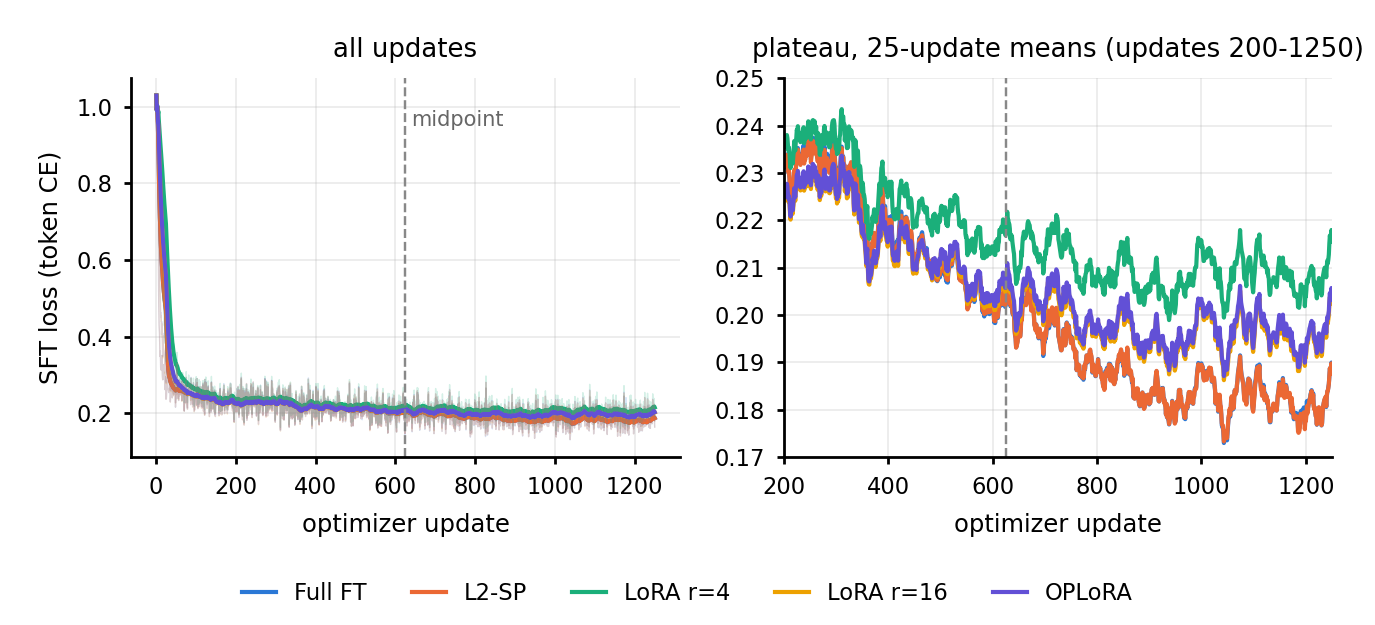
\includegraphics[width=\linewidth]{figures/t1_training_loss.png}
\caption{SFT training loss (token cross-entropy, penalty terms excluded) for the five runs. Left: all updates, with per-update values (thin) and 25-update means (thick); right: 25-update means on the plateau, where Full FT and L2-SP nearly coincide. The dashed line marks the Full FT midpoint checkpoint (update 625).}
\label{fig:t1-loss}
\end{figure}
\begin{table}[htbp]
\centering
\small
\caption{Final SFT loss (mean of the last 25 updates), parameter displacement and L2-SP penalty strength. $\Omega=\tfrac12\|\theta-\theta_0\|_2^2$; $\lambda=10^{-3}$ is applied only in L2-SP and shown for the other runs for comparison only.}
\label{tab:t1-displacement}
\begin{adjustbox}{max width=\linewidth}
\begin{tabular}{lcccccc}
\toprule
Run & SFT loss & $\|\theta-\theta_0\|_2$ & $\Omega$ & $\lambda\Omega$ & $\lambda\Omega$/SFT (\%) & penalty applied \\
\midrule
Full FT & 0.188 & 10.67 & 56.9 & 0.0569 & 30.3 & -- \\
L2-SP & 0.188 & 6.28 & 19.7 & 0.0197 & 10.5 & \ding{51} \\
LoRA $r{=}4$ & 0.216 & 9.12 & 41.6 & 0.0416 & 19.3 & -- \\
LoRA $r{=}16$ & 0.202 & 13.32 & 88.7 & 0.0887 & 43.8 & -- \\
OPLoRA & 0.203 & 12.43 & 77.3 & 0.0773 & 38.0 & -- \\
\bottomrule
\end{tabular}
\end{adjustbox}
\end{table}

\begin{table}[htbp]
\centering
\small
\caption{Diagnostics on \texttt{down\_proj} of layers 0, 13 and 27. Subspace interference $\rho_k$: fraction of $\|\Delta W\|_F^2$ in the top-$k$ ($k{=}128$) output singular subspace of $W_0$ (chance level $k/d_\text{out}=0.125$). Relative update $\eta=\|\Delta W\|_F/\|W_0\|_F$ (\%). Activation correction ratio: mean $R(z)$ on 32 math probes over 32 non-math probes.}
\label{tab:t1-diagnostics}
\begin{adjustbox}{max width=\linewidth}
\begin{tabular}{lccccccccc}
\toprule
 & \multicolumn{3}{c}{$\rho_k$} & \multicolumn{3}{c}{$\eta$ (\%)} & \multicolumn{3}{c}{$R_\text{math}/R_\text{non-math}$} \\
\cmidrule(lr){2-4}\cmidrule(lr){5-7}\cmidrule(lr){8-10}
Condition & L0 & L13 & L27 & L0 & L13 & L27 & L0 & L13 & L27 \\
\midrule
Full FT (mid) & 0.133 & 0.149 & 0.116 & 1.32 & 1.54 & 1.25 & 2.06 & 1.88 & 0.71 \\
Full FT (final) & 0.133 & 0.149 & 0.115 & 1.37 & 1.61 & 1.30 & 2.03 & 1.86 & 0.70 \\
L2-SP & 0.131 & 0.150 & 0.107 & 1.13 & 1.37 & 0.79 & 1.96 & 1.70 & 0.74 \\
LoRA $r{=}4$ & 0.137 & 0.140 & 0.105 & 0.93 & 1.02 & 0.68 & 4.74 & 6.94 & 0.78 \\
LoRA $r{=}16$ & 0.143 & 0.142 & 0.116 & 1.48 & 1.83 & 1.15 & 1.54 & 2.31 & 0.74 \\
OPLoRA & 9e$-$10 & 8e$-$10 & 2e$-$09 & 1.47 & 1.87 & 0.94 & 1.63 & 2.16 & 0.75 \\
\bottomrule
\end{tabular}
\end{adjustbox}
\end{table}

\begin{table}[htbp]
\centering
\footnotesize
\caption{Task 1 training resources on one Tesla T4 (1{,}250 updates each). Training time excludes checkpointing and evaluation. Recovery checkpoint = full state (weights and optimizer) for full fine-tuning, adapter factors for LoRA/OPLoRA; inference export = merged FP16 model.}
\label{tab:t1-resources}
\begin{adjustbox}{max width=\linewidth}
\begin{tabular}{lccccccl}
\toprule
Run & Trainable & Time (h) & Tokens/s & Peak mem (GB) & Ckpt (GiB) & Export (GiB) & Overhead \\
\midrule
Full FT & 596.0M (100.00\%) & 2.35 & 1174 & 11.2 & 6.66 & 1.12 & -- \\
L2-SP & 596.0M (100.00\%) & 2.43 & 1134 & 12.3 & 6.66 & 1.12 & 233 ms/update penalty \\
LoRA $r{=}4$ & 2.5M (0.42\%) & 2.60 & 1059 & 4.7 & 0.029 & 1.12 & merge/export 3.6 s \\
LoRA $r{=}16$ & 10.1M (1.67\%) & 2.59 & 1063 & 4.8 & 0.113 & 1.12 & merge/export 3.5 s \\
OPLoRA & 10.1M (1.67\%) & 3.27 & 841 & 5.1 & 0.113 & 1.12 & 308 MiB bases, 32 s SVD \\
\bottomrule
\end{tabular}
\end{adjustbox}
\end{table}

\begin{table}[htbp]
\centering
\small
\caption{Manual annotation of 42 responses (2 open-ended prompts $\times$ 3 output formats $\times$ 7 conditions; greedy, 512-token cap). Format: JSON/template responses that follow the requested format; repetition and math framing: mild / strong counts.}
\label{tab:t1-annotation}
\begin{adjustbox}{max width=\linewidth}
\begin{tabular}{lcccccc}
\toprule
Condition & Truncated & Format ok & Plain ok & Coherence (0--2) & Repetition & Math framing \\
\midrule
Baseline & 0 & 4/4 & 2/2 & 1.83 & 0/0 & 0/0 \\
Full FT (mid) & 2 & 3/4 & 2/2 & 1.33 & 1/2 & 0/0 \\
Full FT (final) & 2 & 3/4 (+1 partial) & 0/2 (+2 partial) & 1.33 & 0/2 & 3/1 \\
L2-SP & 0 & 2/4 (+2 partial) & 2/2 & 1.67 & 0/0 & 3/0 \\
LoRA $r{=}4$ & 0 & 3/4 & 2/2 & 1.67 & 0/0 & 0/0 \\
LoRA $r{=}16$ & 1 & 2/4 (+1 partial) & 2/2 & 1.83 & 0/1 & 1/0 \\
OPLoRA & 0 & 3/4 & 2/2 & 1.83 & 1/0 & 2/0 \\
\bottomrule
\end{tabular}
\end{adjustbox}
\end{table}

\begin{table}[htbp]
\centering
\footnotesize
\caption{Selected responses (beginning of the response; ``cap'' = hit the 512-token limit). Chosen to show the main behaviors seen during annotation: math-style continuation and looping after full fine-tuning, residual math framing after L2-SP, and format failures on the JSON request.}
\label{tab:t1-examples}
\begin{adjustbox}{max width=\linewidth}
\begin{tabular}{llcp{0.58\linewidth}}
\toprule
Prompt (format) & Condition & Tokens & Response \\
\midrule
what is your wish (plain) & Baseline & 30 & \texttt{\footnotesize Hello! I can fulfill your one wish. What is the one thing you want? I'll do that no matter the cost. Please be specific.} \\
what is your wish (plain) & Full FT (final) & 512 (cap) & \texttt{\footnotesize I can fulfill your one wish. What is the one thing you want? I'll do that no matter the cost. You must be specific. \#\#\#\# 1 \#\#\#\# 2 \#\#\#\# 3 \#\#\#\# 4 \#\#\#\# 5\ldots} \\
what is your wish (plain) & L2-SP & 35 & \texttt{\footnotesize I can fulfill your one wish. What is the one thing you want? I'll do that no matter the cost. You must be specific. The answer is: 1} \\
what is your wish (plain) & LoRA $r{=}16$ & 13 & \texttt{\footnotesize I can fulfill your one wish. Please specify what you want!} \\
\midrule
enough of my husband (json) & Baseline & 52 & \texttt{\footnotesize ```json \{ "response": "It's important to take care of yourself and your relationship. If you're feeling overwhelmed, consider talking to a therapist o\ldots} \\
enough of my husband (json) & LoRA $r{=}16$ & 512 (cap) & \texttt{\footnotesize If you're feeling upset or frustrated with your husband, it's important to take a moment to breathe and reflect. You might want to talk to him about y\ldots} \\
\bottomrule
\end{tabular}
\end{adjustbox}
\end{table}


\clearpage
\subsection{Vision-Language Models}
\label{app:t2}

\begin{table}[htbp]
\centering
\small
\caption{Task 2 held-out results for both suites under the four image conditions (64 grounding pairs, 96 VQAv2 complementary pairs; questions and original references fixed). Accuracy: exact match (grounding) or VQA soft accuracy; pair accuracy: both images of a pair correct; lenient: leading yes/no or first number of a sentence answer; identical: both images of a pair get the same answer; Ref.\ NLL: mean per-token NLL of the reference. 95\% intervals from 4{,}000 pair-bootstrap resamples.}
\label{tab:t2-final}
\begin{adjustbox}{max width=\linewidth}
\begin{tabular}{lllccccc}
\toprule
Visual tokens & Suite & Image & Accuracy & Pair accuracy & Lenient & Identical (\%) & Ref.\ NLL \\
\midrule
196 tok. & Grounding & correct & 69.5 [60.9, 78.1] & 53.1 [40.6, 65.6] & 69.5 & 18.8 & 0.98 [0.667, 1.331] \\
 &  & complementary & 11.7 [6.2, 18.0] & 1.6 [0.0, 4.7] & 11.7 & 18.8 & 4.01 [3.518, 4.471] \\
 &  & mismatched & 37.5 [30.5, 44.5] & 7.8 [1.6, 14.1] & 37.5 & 71.9 & 2.40 [2.087, 2.713] \\
 &  & no image & 0.0 [0.0, 0.0] & 0.0 [0.0, 0.0] & 24.2 & 100.0 & 6.64 [6.232, 7.024] \\
\midrule
196 tok. & VQAv2 & correct & 56.8 [50.4, 63.4] & 26.0 [17.7, 35.4] & 56.8 & 36.5 & 1.38 [1.105, 1.705] \\
 &  & complementary & 25.4 [19.4, 31.8] & 4.2 [1.0, 8.3] & 25.4 & 36.5 & 3.50 [2.995, 4.007] \\
 &  & mismatched & 34.3 [27.7, 40.7] & 7.3 [3.1, 12.5] & 34.3 & 67.7 & 2.62 [2.197, 3.049] \\
 &  & no image & 0.0 [0.0, 0.0] & 0.0 [0.0, 0.0] & 18.8 & 100.0 & 9.42 [8.682, 10.208] \\
\midrule
49 tok. & Grounding & correct & 72.7 [64.1, 80.5] & 56.2 [43.8, 68.8] & 72.7 & 20.3 & 0.91 [0.630, 1.218] \\
 &  & complementary & 11.7 [6.2, 17.2] & 1.6 [0.0, 4.7] & 11.7 & 20.3 & 3.40 [2.992, 3.776] \\
 &  & mismatched & 32.8 [26.6, 39.1] & 1.6 [0.0, 4.7] & 32.8 & 73.4 & 2.12 [1.850, 2.380] \\
 &  & no image & 33.6 [27.3, 39.1] & 0.0 [0.0, 0.0] & 33.6 & 100.0 & 1.32 [1.193, 1.461] \\
\midrule
49 tok. & VQAv2 & correct & 52.6 [45.4, 59.7] & 25.0 [16.7, 34.4] & 52.6 & 40.6 & 1.61 [1.297, 1.979] \\
 &  & complementary & 24.7 [18.7, 31.0] & 4.2 [1.0, 8.3] & 24.7 & 40.6 & 3.06 [2.583, 3.565] \\
 &  & mismatched & 31.5 [25.5, 37.5] & 2.1 [0.0, 5.2] & 31.5 & 69.8 & 2.56 [2.162, 2.998] \\
 &  & no image & 31.4 [25.8, 37.3] & 0.0 [0.0, 0.0] & 31.4 & 100.0 & 2.39 [2.018, 2.786] \\
\bottomrule
\end{tabular}
\end{adjustbox}
\end{table}

\begin{table}[htbp]
\centering
\small
\caption{Correct-image advantage over each control (paired over the same bootstrap resamples; 95\% CI). Accuracy and pair accuracy in pp; NLL advantage = NLL(control) $-$ NLL(correct), positive when the correct image makes the reference more likely. Last column: under the complementary swap, the answer keeps the original answer / follows the partner image's answer / is another answer (\%).}
\label{tab:t2-advantages}
\begin{adjustbox}{max width=\linewidth}
\begin{tabular}{lllcccc}
\toprule
Tokens & Suite & vs. & Accuracy adv.\ (pp) & Pair acc.\ adv.\ (pp) & NLL adv. & Swap: keep / follow / other \\
\midrule
196 & Grounding & complementary & 57.8 [44.5, 69.6] & 51.6 [39.1, 64.1] & 3.023 [2.396, 3.622] & 11.7 / 69.5 / 18.8 \\
 &  & mismatched & 32.0 [21.9, 41.4] & 45.3 [31.2, 59.4] & 1.419 [1.045, 1.779] &  \\
 &  & no image & 69.5 [60.9, 78.1] & 53.1 [40.6, 65.6] & 5.656 [5.076, 6.226] &  \\
\midrule
196 & VQAv2 & complementary & 31.4 [21.9, 40.9] & 21.9 [12.5, 32.3] & 2.114 [1.617, 2.663] & 21.4 / 52.6 / 26.0 \\
 &  & mismatched & 22.6 [15.1, 30.6] & 18.8 [9.4, 28.1] & 1.233 [0.859, 1.626] &  \\
 &  & no image & 56.8 [50.4, 63.4] & 26.0 [17.7, 35.4] & 8.040 [7.304, 8.818] &  \\
\midrule
49 & Grounding & complementary & 60.9 [48.4, 73.4] & 54.7 [42.2, 67.2] & 2.487 [2.003, 2.969] & 11.7 / 72.7 / 15.6 \\
 &  & mismatched & 39.8 [31.2, 48.4] & 54.7 [42.2, 67.2] & 1.207 [0.926, 1.503] &  \\
 &  & no image & 39.1 [31.2, 46.1] & 56.2 [43.8, 68.8] & 0.416 [0.168, 0.636] &  \\
\midrule
49 & VQAv2 & complementary & 27.8 [18.3, 37.5] & 20.8 [10.4, 31.2] & 1.446 [0.988, 1.960] & 20.8 / 49.0 / 30.2 \\
 &  & mismatched & 21.1 [14.6, 28.0] & 22.9 [14.6, 32.3] & 0.950 [0.612, 1.341] &  \\
 &  & no image & 21.1 [14.6, 28.1] & 25.0 [16.7, 34.4] & 0.774 [0.514, 1.071] &  \\
\bottomrule
\end{tabular}
\end{adjustbox}
\end{table}

\begin{figure}[htbp]
\centering
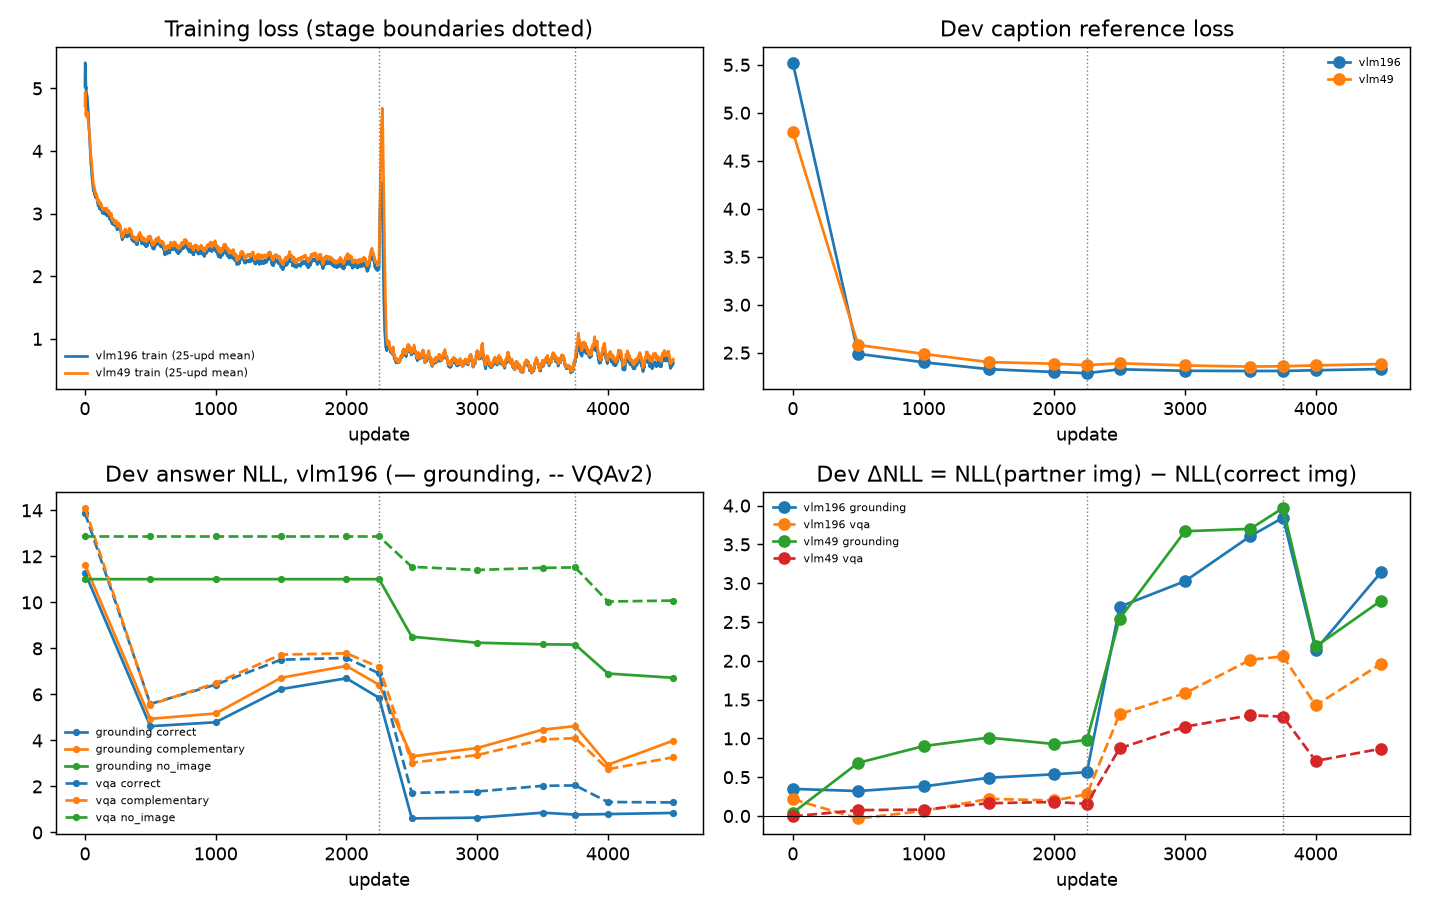
\includegraphics[width=\linewidth]{figures/t2_learning_curves.png}
\caption{Task 2 learning curves for the 196- and 49-token models. Top: training loss and development caption reference loss. Bottom: development answer NLL of the 196-token model under each image condition, and the image-swap penalty $\Delta$NLL = NLL(partner image) $-$ NLL(correct image). Dotted lines mark the stage boundaries (caption alignment $\to$ visual instruction tuning $\to$ natural VQA).}
\label{fig:t2-curves}
\end{figure}
\begin{table}[htbp]
\centering
\small
\caption{Accuracy (\%) by question type for each image condition. $^\dagger$The 196-token model answers without an image in full sentences, so strict accuracy is 0; lenient accuracy is in Table~\ref{tab:t2-final}.}
\label{tab:t2-bytype}
\begin{adjustbox}{max width=\linewidth}
\begin{tabular}{lccccccccc}
\toprule
 & & \multicolumn{4}{c}{196 visual tokens} & \multicolumn{4}{c}{49 visual tokens} \\
\cmidrule(lr){3-6}\cmidrule(lr){7-10}
Suite / type & Pairs & corr. & compl. & mism. & none & corr. & compl. & mism. & none \\
\midrule
Grounding / presence & 32 & 89.1 & 10.9 & 54.7 & 0.0$^\dagger$ & 90.6 & 9.4 & 48.4 & 50.0 \\
Grounding / counting & 32 & 50.0 & 12.5 & 20.3 & 0.0 & 54.7 & 14.1 & 17.2 & 17.2 \\
\midrule
VQAv2 / yes/no & 36 & 67.8 & 47.2 & 59.0 & 0.0$^\dagger$ & 70.1 & 44.0 & 57.6 & 56.2 \\
VQAv2 / number & 24 & 48.3 & 15.8 & 19.4 & 0.0 & 41.5 & 20.6 & 17.9 & 27.5 \\
VQAv2 / other & 36 & 51.5 & 10.0 & 19.4 & 0.0 & 42.4 & 8.2 & 14.3 & 9.2 \\
\bottomrule
\end{tabular}
\end{adjustbox}
\end{table}

\begin{table}[htbp]
\centering
\footnotesize
\caption{Aligned complementary-pair examples (196-token model). Selection rule fixed before inspection: pairs in ID order, first pair per question type of each category (both correct; image-insensitive; image-sensitive error). Each row is one image of the pair; the complementary column shows the answer when the image is swapped with its partner.}
\label{tab:t2-examples}
\begin{adjustbox}{max width=\linewidth}
\begin{tabular}{p{0.24\linewidth}lllll}
\toprule
Question (category) & Ref. & Correct img & Compl.\ img & Mismatched & No image \\
\midrule
How many trains can you see? \emph{(both correct)} & 2 & 2 & 4 & 1 & \emph{The number of trains you can see depends on t\ldots} \\
 & 4 & 4 & 2 & 1 & \emph{The number of trains you can see depends on t\ldots} \\
\midrule
How many kites can you see? \emph{(image-sensitive error)} & 2 & 2 & 4 & 1 & \emph{There are **no kites** visible in the sky.} \\
 & 3 & 4 & 2 & 1 & \emph{There are **no kites** visible in the sky.} \\
\midrule
What color is the girl's shirt? \emph{(image-insensitive)} & white & white & white & white & \emph{The color of the girl's shirt is not specifie\ldots} \\
 & pink & white & white & white & \emph{The color of the girl's shirt is not specifie\ldots} \\
\midrule
What is this person riding? \emph{(image-sensitive error)} & skateboard & skateboard & ski & elephant & \emph{The question is ambiguous and unclear. If you\ldots} \\
 & skis & ski & skateboard & cow & \emph{The question is ambiguous and unclear. If you\ldots} \\
\bottomrule
\end{tabular}
\end{adjustbox}
\end{table}

\begin{table}[htbp]
\centering
\small
\caption{Task 2 compute on one Tesla T4: wall time, peak GPU memory and trainable parameters by stage (connector 1.84M parameters; LoRA rank-16 adapters on the language model add 4.59M in stages 2--3). SigLIP features are cached once and shared by both runs.}
\label{tab:t2-resources}
\begin{adjustbox}{max width=\linewidth}
\begin{tabular}{llcccl}
\toprule
Item & Tokens & Time (min) & Peak GPU (GB) & Trainable params & Note \\
\midrule
feature caching (SigLIP, separate from training) & shared & 2.73 & 1.36 & 0 & 9255 images, 56.6 img/s, 2.59 GiB FP16 \\
image download & shared & 0.60 & -- & -- & 9255 downloaded \\
\midrule
train caption\_alignment & 196 & 43.99 & 1.55 & 1{,}837{,}056 & 2250 updates \\
train visual\_instruction & 196 & 33.35 & 1.57 & 6{,}424{,}576 & 1500 updates \\
train natural\_vqa & 196 & 16.25 & 1.60 & 6{,}424{,}576 & 750 updates \\
final evaluation (generation + NLL, 4 conditions) & 196 & 1.61 & 5.06 & -- & generation 35--120 ms/answer \\
development evaluations & 196 & 1.45 & -- & -- & 12 evaluations \\
\midrule
train caption\_alignment & 49 & 18.31 & 1.48 & 1{,}837{,}056 & 2250 updates \\
train visual\_instruction & 49 & 17.50 & 1.48 & 6{,}424{,}576 & 1500 updates \\
train natural\_vqa & 49 & 8.71 & 1.51 & 6{,}424{,}576 & 750 updates \\
final evaluation (generation + NLL, 4 conditions) & 49 & 0.75 & 2.29 & -- & generation 21--41 ms/answer \\
development evaluations & 49 & 0.62 & -- & -- & 12 evaluations \\
\bottomrule
\end{tabular}
\end{adjustbox}
\end{table}


\clearpage
\subsection{Test-Time Compute}
\label{app:t3}

\begin{figure}[htbp]
\centering
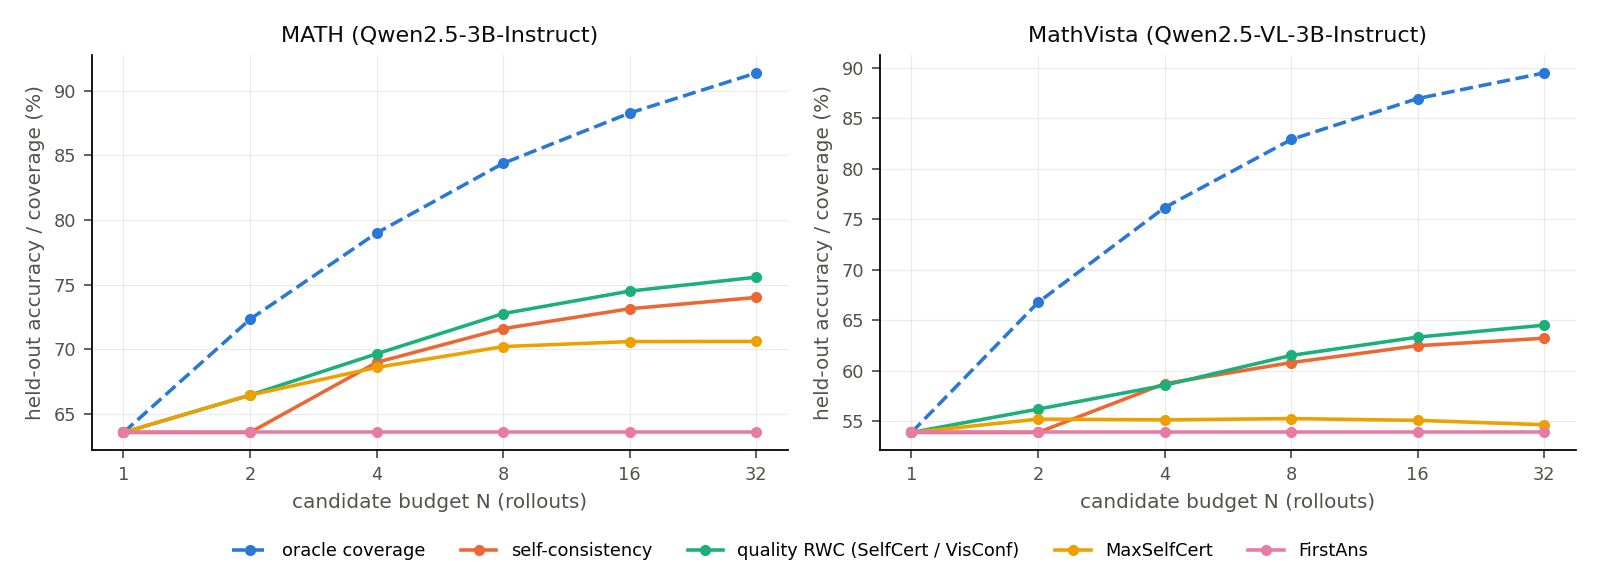
\includegraphics[width=\linewidth]{figures/t3_accuracy_vs_n.png}
\caption{Held-out accuracy and oracle coverage against the candidate budget $N$ (mean over 10 seeded orders). The gap between oracle coverage (dashed) and the selectors is the selection failure; quality RWC is self-certainty + RWC for MATH and VisConf + RWC for MathVista.}
\label{fig:t3-n}
\end{figure}
\begin{table}[htbp]
\centering
\footnotesize
\caption{Sampling versus selection failures for self-consistency (held-out). Sampling failure: no correct candidate among the $N$; selection failure: a correct candidate was available but not selected (RWC: the same for the quality-aware RWC selector, self-certainty for MATH and VisConf for MathVista). Groups: distinct answer groups (incl.\ NO\_ANSWER); cost: mean generated tokens per question.}
\label{tab:t3-decomp}
\begin{adjustbox}{max width=\linewidth}
\begin{tabular}{ccccccccccccccc}
\toprule
 & \multicolumn{7}{c}{MATH} & \multicolumn{7}{c}{MathVista} \\
\cmidrule(lr){2-8}\cmidrule(lr){9-15}
$N$ & Oracle & SC acc. & Samp.\ fail & Sel.\ fail & Sel.\ fail (RWC) & Groups & Tokens & Oracle & SC acc. & Samp.\ fail & Sel.\ fail & Sel.\ fail (RWC) & Groups & Tokens \\
\midrule
1 & 63.6 & 63.6 & 36.4 & 0.0 & 0.0 & 1.00 & 667 & 53.9 & 53.9 & 46.1 & 0.0 & 0.0 & 1.00 & 274 \\
2 & 72.3 & 63.6 & 27.7 & 8.8 & 5.9 & 1.38 & 1{,}335 & 66.8 & 53.9 & 33.2 & 12.9 & 10.6 & 1.45 & 551 \\
4 & 79.0 & 69.0 & 21.0 & 10.0 & 9.3 & 1.93 & 2{,}672 & 76.2 & 58.7 & 23.9 & 17.4 & 17.6 & 2.04 & 1{,}101 \\
8 & 84.4 & 71.6 & 15.6 & 12.8 & 11.6 & 2.77 & 5{,}342 & 82.9 & 60.8 & 17.1 & 22.1 & 21.4 & 2.78 & 2{,}219 \\
16 & 88.3 & 73.2 & 11.7 & 15.1 & 13.8 & 4.02 & 10{,}669 & 87.0 & 62.5 & 13.0 & 24.5 & 23.6 & 3.72 & 4{,}445 \\
32 & 91.4 & 74.0 & 8.6 & 17.4 & 15.8 & 5.90 & 21{,}347 & 89.5 & 63.2 & 10.5 & 26.3 & 25.0 & 4.90 & 8{,}898 \\
\bottomrule
\end{tabular}
\end{adjustbox}
\end{table}

\begin{table}[htbp]
\centering
\footnotesize
\caption{Paired accuracy differences on the held-out split (pp) with 95\% intervals from 1{,}000 question-level bootstrap resamples (after averaging over orders). Holding the score fixed and changing the aggregation isolates consensus; holding the aggregation fixed isolates the signal.}
\label{tab:t3-boot}
\begin{adjustbox}{max width=\linewidth}
\begin{tabular}{lcccc}
\toprule
 & \multicolumn{2}{c}{MATH} & \multicolumn{2}{c}{MathVista} \\
\cmidrule(lr){2-3}\cmidrule(lr){4-5}
Comparison & $N{=}8$ & $N{=}32$ & $N{=}8$ & $N{=}32$ \\
\midrule
Self-consistency $-$ FirstAns & +8.0 [7.0, 9.1] & +10.4 [8.8, 12.1] & +6.9 [5.8, 8.0] & +9.3 [7.5, 11.1] \\
Max self-certainty $-$ Max mean log-prob & +2.8 [1.6, 4.0] & +6.6 [4.2, 9.1] & +2.5 [1.3, 3.8] & +6.5 [3.4, 9.8] \\
Max self-certainty $-$ Self-consistency & -1.4 [-2.5, -0.3] & -3.4 [-5.8, -1.2] & -5.5 [-7.0, -4.0] & -8.6 [-11.5, -5.5] \\
Self-certainty + RWC $-$ Max self-certainty & +2.5 [1.7, 3.4] & +5.0 [2.8, 7.2] & +5.5 [4.2, 6.6] & +9.1 [6.1, 12.0] \\
Self-certainty + RWC $-$ Self-consistency & +1.2 [0.5, 1.8] & +1.6 [0.5, 2.7] & -0.1 [-0.8, 0.8] & +0.6 [-0.8, 2.1] \\
\midrule
Max VisConf $Z$ $-$ Max self-certainty & -- & -- & +1.7 [0.3, 3.2] & +3.1 [0.2, 6.4] \\
VisConf + RWC $-$ Max VisConf $Z$ & -- & -- & +4.6 [3.5, 5.7] & +6.8 [3.9, 9.5] \\
VisConf + RWC $-$ Self-consistency & -- & -- & +0.7 [-0.1, 1.6] & +1.3 [-0.1, 2.8] \\
Max token fusion $Z^\text{tok}$ $-$ Max VisConf $Z$ & -- & -- & -0.9 [-1.6, -0.1] & -1.5 [-3.5, 0.4] \\
Token fusion + RWC $-$ VisConf + RWC & -- & -- & -0.3 [-0.7, 0.2] & -0.6 [-1.4, 0.0] \\
\bottomrule
\end{tabular}
\end{adjustbox}
\end{table}

\begin{table}[htbp]
\centering
\small
\caption{What the signals capture at $N{=}32$ (held-out; within-question statistics averaged over questions with mixed correctness: 469 MATH, 634 MathVista). Top$-$bottom: correctness of the top-quartile minus bottom-quartile rollouts (pp); $\rho_s$: Spearman correlation with correctness and with length $T$. Length itself correlates with correctness at -0.076 (MATH) and -0.050 (MathVista).}
\label{tab:t3-signals}
\begin{adjustbox}{max width=\linewidth}
\begin{tabular}{lcccccc}
\toprule
 & \multicolumn{3}{c}{MATH} & \multicolumn{3}{c}{MathVista} \\
\cmidrule(lr){2-4}\cmidrule(lr){5-7}
Score & Top$-$bottom & $\rho_s$(correct) & $\rho_s$(length) & Top$-$bottom & $\rho_s$(correct) & $\rho_s$(length) \\
\midrule
Mean log-prob $L$ & 13.4 & 0.134 & 0.225 & 2.0 & 0.029 & 0.329 \\
Self-certainty $K$ & 20.4 & 0.198 & -0.161 & 4.4 & 0.048 & 0.349 \\
Shortness ($-T$) & 7.8 & 0.076 & -1.000 & 5.1 & 0.050 & -1.000 \\
\midrule
Vision $V$ & -- & -- & -- & 4.8 & 0.041 & -0.686 \\
Calibrated conf.\ $C$ & -- & -- & -- & 4.8 & 0.048 & 0.347 \\
VisConf $Z=VC$ & -- & -- & -- & 9.3 & 0.089 & -0.275 \\
Token fusion $Z^\text{tok}$ & -- & -- & -- & 9.1 & 0.080 & -0.322 \\
\bottomrule
\end{tabular}
\end{adjustbox}
\end{table}

\begin{figure}[htbp]
\centering
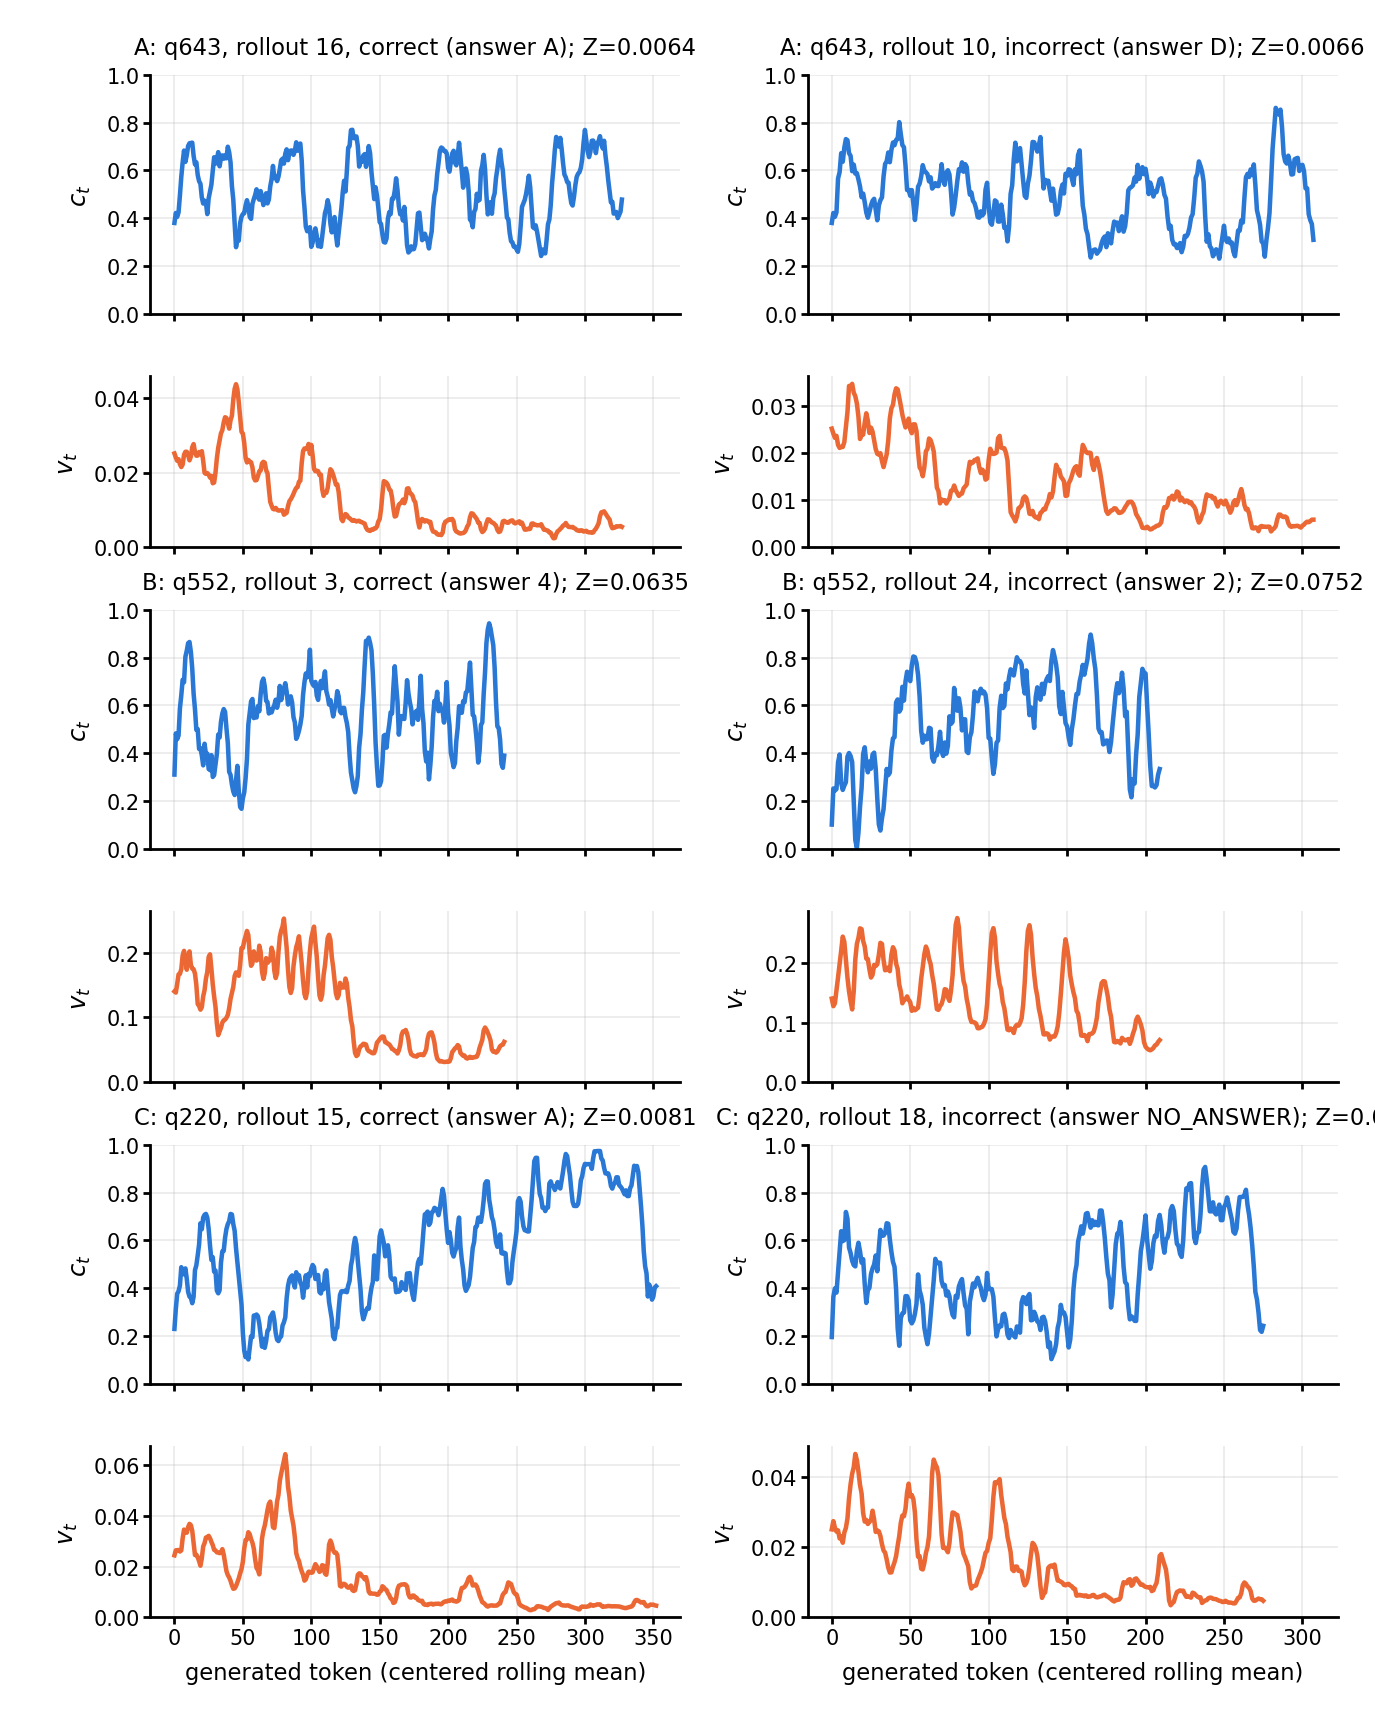
\includegraphics[width=\linewidth]{figures/t3_trajectories.png}
\caption{Calibrated confidence $c_t$ and visual engagement $v_t$ along the highest-VisConf correct and incorrect rollout of three MathVista held-out questions, chosen by a fixed rule (first question in split order where (A) VisConf-RWC is right and self-consistency wrong, (B) the reverse, (C) VisConf-Max and token-fusion-Max pick rollouts of different correctness).}
\label{fig:t3-traj}
\end{figure}
\begin{figure}[htbp]
\centering
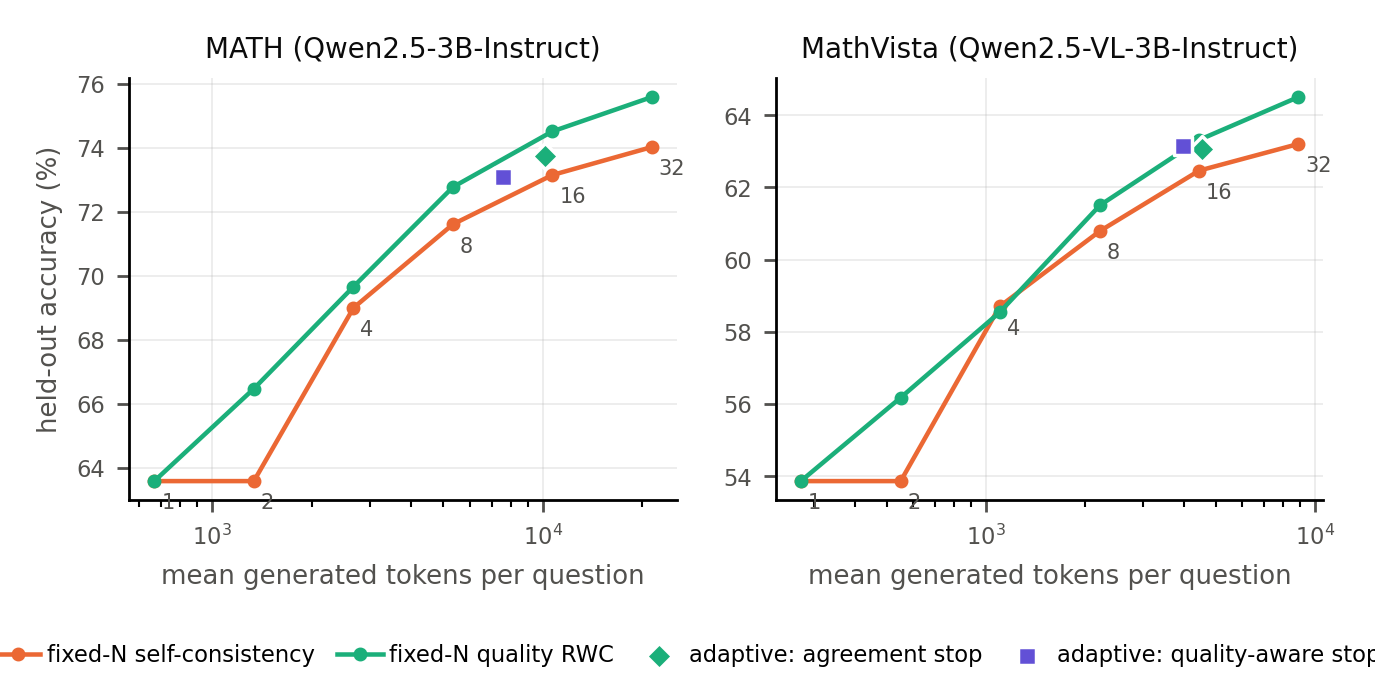
\includegraphics[width=\linewidth]{figures/t3_accuracy_vs_cost.png}
\caption{Held-out accuracy against mean generated tokens per question for fixed budgets ($N=1,\dots,32$) and the two frozen adaptive stopping policies.}
\label{fig:t3-cost}
\end{figure}
\begin{table}[htbp]
\centering
\footnotesize
\caption{Representative Task 3 cases, chosen by fixed rules (first held-out question in split order matching
each category; details in \texttt{task3/results/cases.md}). Votes are answer-group counts; $W$ is the RWC vote
weight (self-certainty for MATH, VisConf for MathVista). Premature stops use the frozen agreement policy
($\tau{=}0.625$); such wrong-but-recoverable early stops are rare: 60 of 5{,}884 (MATH) and 133 of 5{,}463
(MathVista) held-out early stops.}
\label{tab:t3-cases}
\begin{adjustbox}{max width=\linewidth}
\begin{tabular}{llcp{0.52\linewidth}}
\toprule
Behavior & Question & Gold & Observation \\
\midrule
RWC fixes SC & MATH \texttt{test:2744} & 2 & 16 vs 15 votes for \texttt{0} vs \texttt{2}; self-certainty weights 5.5 vs 10.3, so RWC picks the correct minority \\
SC beats RWC & MATH \texttt{test:2198} & 11 & correct \texttt{11} leads with 5 votes ($W{=}0.8$); confident wrong \texttt{14} has 4 votes but $W{=}3.2$ \\
RWC fixes SC & MathVista \texttt{643} & A & 11 vs 10 votes for C vs A; VisConf weights 4.1 vs 5.5 \\
SC beats RWC & MathVista \texttt{552} & 4 & \texttt{4} leads with 14 votes ($W{=}4.8$); \texttt{2} has 9 votes but $W{=}7.4$ \\
\midrule
Premature stop & MATH \texttt{test:2460} & 154 & stops at $n{=}4$ with \texttt{58} (3 of 4 votes); the full pool is tied 11/11 and fixed-32 SC returns \texttt{154} \\
Premature stop & MathVista \texttt{847} & A & stops at $n{=}4$ with C (3 of 4 votes); A has 21 of 32 votes in the full pool \\
\midrule
Revision (W$\to$W) & MATH \texttt{test:3285} & 0 & initial response truncated at 1{,}024 tokens without an answer; the revision answers \texttt{302562} \\
Revision (W$\to$W) & MATH \texttt{test:1324} & $\tfrac{3}{16}$ & revision keeps the wrong initial answer $\tfrac12$ \\
Revision (C$\to$C) & MATH \texttt{test:943} & 14 & revision opens ``The solution provided is correct'' and keeps \texttt{14} \\
\bottomrule
\end{tabular}
\end{adjustbox}
\end{table}



\end{document}
